\documentclass[8pt]{beamer}
\mode<presentation>
{
  % https://deic-web.uab.cat/~iblanes/beamer_gallery/index.html
  \usetheme{Rochester}
  \usefonttheme{default}
  \usecolortheme{whale}
}
\renewcommand{\baselinestretch}{1.35}
%\usepackage[legalpaper, landscape, margin=2in]{geometry}
\usepackage[utf8]{inputenc}
\usepackage[T1]{fontenc}
\usepackage{tikz}
\usepackage{circuitikz}
\usepackage{hyperref}
\usepackage{listings}
\usepackage{multicol}
\usepackage{listings}
\usepackage{tikz}
\usepackage{graphicx}
\usepackage{array}
\usepackage{tabularx}
\usetikzlibrary{shapes,arrows}
\setlength{\columnsep}{4.5cm}

\title[Report]{EE4015 Assignment-1 Presentation}
\author{Krishna Srikar Durbha (EE18BTECH11014)}
\date{$25^{\text{th}}$ August 2021}

\begin{document}
\begin{frame}
  \titlepage
\end{frame}

\begin{frame}[fragile]{Question}
Consider the following ANSI C function:
\begin{lstlisting}[language=C]
int SomeFunction(int x, int y){
	if ((x == 1) || (y == 1)) return 1;
	if (x == y) return x;
	if (x > y) return SomeFunction(x-y, y);
	if (x < y) return SomeFunction(x, y-x);
}
\end{lstlisting}
The value of returned by SomeFunction(15,255) is \rule{1cm}{0.15mm}
\end{frame}

\section{Euclidean Algorithm by Subtraction}
\begin{frame}[allowframebreaks]{Euclidean Algorithm by Subtraction}
Euclidean Algorithm is a recursive method of finding Greatest Common Divisor of 2 numbers. For some positive integers $a$ and $b$, it works by repeatedly subtracting the smaller number from the larger one until they become equal. At this point, the value of either term is the greatest common divisor of our inputs.

\textbf{Algorithm:}\\
Step-1: If $a = b$, then return the value of a\\
Step-2: Otherwise, if a > b then let a = a - b and return to Step-1\\
Step-3: Otherwise, if a < b, then let b = b - a and return to Step-1\\

\vspace{0.2in}

\textbf{Proof}:\\
Proof involves proving that, subtracting between $a$ and $b$ doesn't change GCD. Let $a$, $b$ be 2 positive integers such that $gcd(a,b) = m$ and $a > b$. So, it can be written as,
\begin{align}
    a = a_{1} \times m \\
    b = b_{1} \times m \\
    gcd(a,b) = m \implies gcd(a_{1}, b_{1}) = 1
\end{align}

\framebreak
We need to prove that $gcd(a-b,b) = m$. We will prove it by contradiction. Let $gcd(a-b,b) = M$ where $M > m \implies  k \neq 1$
\begin{align}
    a-b = (a_{1} - b_{1}) \times m\\
    b =  b_{1} \times m\\
    gcd(a-b,b) = M \implies M = k \times m \text{ (For some integer $k$)}\\
    a-b \equiv 0\ (\textrm{mod}\ M) \text{ and } b \equiv 0\ (\textrm{mod}\ M)\\
    \implies a-b \equiv 0\ (\textrm{mod}\ km) \text{ and } b \equiv 0\ (\textrm{mod}\ km)\\
    \implies a_{1} - b_{1} \equiv 0\ (\textrm{mod}\ k) \text{ and } b_{1} \equiv 0\ (\textrm{mod}\ k)\\
    \implies a_{1} \equiv 0\ (\textrm{mod}\ k) \text{ and } b_{1} \equiv 0\ (\textrm{mod}\ k)
\end{align}
We know that $gcd(a_{1}, b_{1}) = 1$, so there doesn't exist a $M \neq m$ such that $gcd(a-b, b) = M$. So, from contradiction, $gcd(a, b) = gcd(a-b, b) = M$ for $a > b$. Worst Case Time-Complexity is $\mathcal{O}(a+b)$.

So, the solution to the given question is:
\[
\begin{split}
&f(15,255) = f(15,240) = f(15,225) = f(15,210)\\
&= f(15,195) = f(15,180) = f(15,165) = f(15,150)\\
&= f(15,135) = f(15,120) = f(15,105) = f(15,90)\\
&= f(15,75) = f(15,60) = f(15,45) = f(15,30)\\
&= f(15,15) = 1
\end{split}\]

\end{frame}

\section{Complexity Analysis of Euclidean Algorithm by Subtraction}
\begin{frame}[allowframebreaks]{Complexity Analysis of Euclidean Algorithm by Subtraction}
Let $a > b$ and $T(n)$ denote time complexity of $gcd(a,b)$ where $n = a+b$. Then,
\begin{align}
T(n) = 1 + T(n-b)\\
T(n-b) = 1 + T(n-2b) \text{ if $a > 2b$}\\
T(n-b) = 1 + T(n-a-b) \text{ if $b < a < 2b$}
\end{align}

On assuming $n > (x_{1}a + x_{2}b)$ for some $x_{1}, x_{2}$, $T(n)$ can be written as:
\begin{align}
T(n) = k + T(n - x_{1}a - x_{2}b) \text{ (For $k = x_{1} + x_{2}$)}
\end{align}
No.of steps vary linearly with $n=a+b$. So, in the worst-case scenerio the algorithm performs $a+b$ subtractions. Hence Worst Case Time-Complexity for calculating GCD of $a$ and  $b$ using Euclidean Algorithm by Subtraction is $\mathcal{O}(a + b)$.\\

\framebreak

\begin{figure}[!ht]
	\centering
	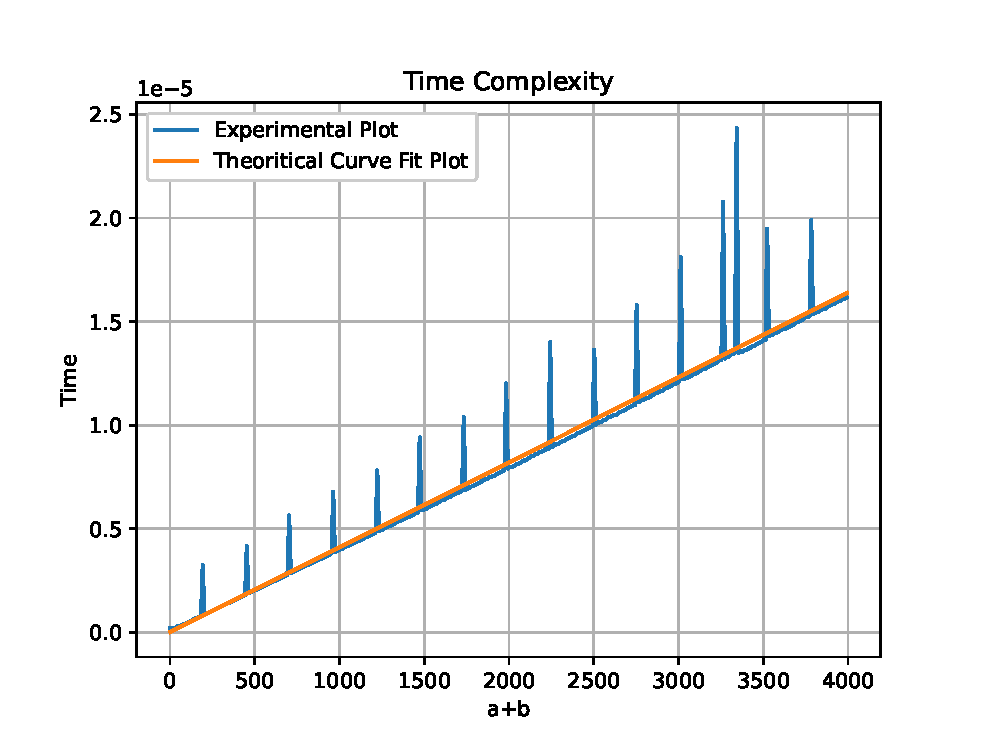
\includegraphics[scale=0.5]{figs/Euclid_Subtraction.eps}
	\caption{Plot of Worst-Case Time Complexity of Euclidean Algorithm by Subtraction}
	\label{fig:0}
\end{figure}


\end{frame}

\section{Euclidean Algorithm by Division}
\begin{frame}[allowframebreaks]{Euclidean Algorithm by Division}
Euclidean Algorithm by Division involves divison rather than subtraction. For some positive integers $a$ and $b$, $gcd(a, b) = gcd(b, a \textrm{ mod}\ b)$. We repeat the procedure until convergence.\\

 Let $a$, $b$ be 2 positive integers such that $a > b$. By applying Euclid's Algorithm from $0^{th}$-step ,
 \begin{align}
     a = q_{0}b + r_{0}\label{eq:ED1}\\
     b = q_{1}r_{0} + r_{1}\\
     r_{0} = q_{2}r_{1} + r_{2}\\
     r_{1} = q_{3}r_{2} + r_{3}...
 \end{align}
 Here $a > b$, $ b > r_{0}$, $r_{0} > r_{1}$, $r_{1} > r_{2}$.. and so on. So, remainders are decreasing after each step.
 
 \framebreak
 
 Let at $n^{th}$-step $r_{n-2} = q_{n}r_{n-1}$ i.e $r_{n} = 0$.
 \begin{align}
    r_{n-2} = q_{n}r_{n-1}\label{eq:ED2}\\
    r_{n-3} = q_{n-1}r_{n-2} + r_{n-1}\\
    \implies r_{n-1} \text{ divides } r_{n-2}, r_{n-3}, r_{n-4},..., r_{1}, r_{0}, b, a\\
    \implies a \equiv 0\ (\textrm{mod}\ r_{n-1}) \text{ and } b \equiv 0\ (\textrm{mod}\ r_{n-1})
\end{align}
So, the proof goes as $gcd(a,b) = r_{n-1}$. We will prove it by contraction. Let  $gcd(a,b) = M \implies M > r_{n-1}$,

\begin{align}
    a = a_{1} \times M \text{ and } b = b_{1} \times M\\
    r_{0} = a - q_{0}b = M(a_{1} - q_{0}b_{1})\\
    r_{1} = b - q_{1}r{0} = M(b_{1} - a_{1} + q_{0}b_{1})
\end{align}

\framebreak

So, M divides $a, b, r_{0}, r_{1}, ... $ and so on all the following remainders. So, $M$ should divide $r_{n-1}$, which implies $r_{n-1} \geq M$ which is a contraction from $M > r_{n-1}$.\\
\vspace{0.2in}
So, there doesn't exist a $M > r_{n-1}$ which is a divisor of $a$ and $b$. So, $gcd(a,b)  = r_{n-1}$.\\
\vspace{0.2in}
So, the solution the given question using Euclidean Algorithm by Divsion is:
\[
\begin{split}
&gcd(15,255) = gcd(255,15) = gcd(15,0) = 15
\end{split}\]

\end{frame}

\section{Complexity Analysis of Euclidean Algorithm by Divsion}
\begin{frame}[allowframebreaks]{Complexity Analysis of Euclidean Algorithm by Division}

Let $f_{n}$ denote elements in Pingala Sequence starting from $n=0$ where $f_{0} = 0, f_{1} = 1, f_{2} = 1,...$ and so on. Elements of the sequence can be written as follows:
\begin{align*}
f_{n+2} = 1 \times f_{n+1} + f_{n}\\
f_{n+1} = 1 \times f_{n} + f_{n-1}\\
...........................\\
f_{4} = 1 \times f_{3} + f_{2}\\
f_{3} = 2 \times f_{2}
\end{align*}
The above equations are similar to equations in Euclidean Algorithm by Division i.e from \eqref{eq:ED1} to \eqref{eq:ED2}. Hence it can be proved that $gcd(f_{n+2}, f_{n+1}) = f_{2} = 1$ and takes $n$ steps to converge.\\

\framebreak

If $gcd(a,b)$ where $a>b$ takes $n$ steps to converge by using Euclidean Algorithm by Division, then $a \geq f_{n+2}$ and $b \geq f_{n+1}$.\\

\textbf{Proof by Mathematical Induction:}\\
Let $a = 2$ and $b = 1$. Then, $gcd(2,1) = 1$ takes $1$ step to converge. $a \geq f_{3} = 2$ and $b \geq f_{2} = 1$. Assuming statements hold true at ${n-1}^{th}$ step, $gcd(b,a\%b)$ takes $n-1$ steps to converge.
\begin{align}
b \geq f_{n+1} \text{ and } a\%b \geq f_{n}\\
a = q_{0}b + a\%b\\
a \geq b + a\%b\\
a \geq f_{n+1} + f_{n} \implies a \geq f_{n+2} \\
\implies a \geq f_{n+2} \text{ and } b \geq f_{n+1}
\end{align}
Hence proved.\\

Let $gcd(a,b)$ takes $n$ steps to converge. Then,
\begin{align}
a \geq f_{n+2}\\
b \geq f_{n+1}\\
f_{n}=\frac{1}{\sqrt{5}}\left(\left(\frac{1+\sqrt{5}}{2}\right)^{n}-\left(\frac{1-\sqrt{5}}{2}\right)^{n}\right)\\
\phi = \frac{1+\sqrt{5}}{2}\\
f_{n} \approx \phi^{n}\\
b \approx \phi^{n+1}\\
n \approx \log_{\phi}{\left(min(a,b)\right)}
\end{align}
So, in the worst-case scenerio the algorithm performs $n \approx \log_{\phi}{\left(min(a,b)\right)} $ divisons. Hence, Worst Case Time-Complexity for calculating GCD of $a$ and  $b$ using Euclidean Algorithm by Division is $\mathcal{O}(\log min(a,b))$.\\

\framebreak

\begin{figure}[!ht]
	\centering
	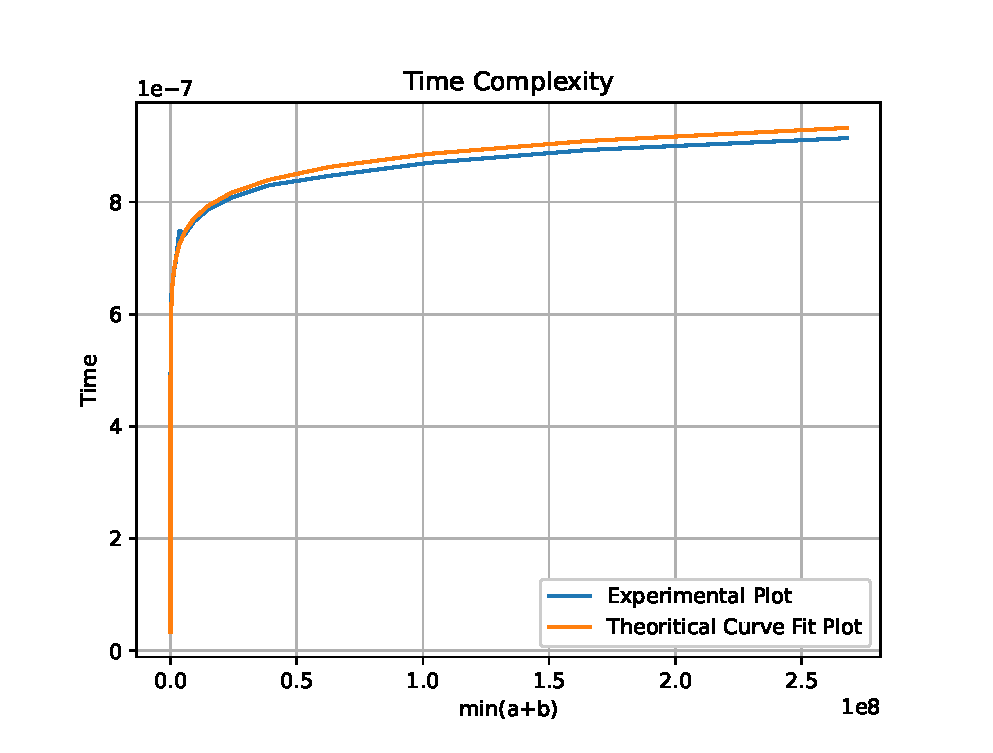
\includegraphics[width=\columnwidth]{figs/Euclid_Division.eps}
	\caption{Plot of Worst-Case Time Complexity of Euclidean Algorithm by Division}
	\label{fig:1}
\end{figure}

\end{frame}

\begin{frame}[allowframebreaks]{Comparison of Algorithms:}
The following example illustrates the difference in no.of steps between Euclidean Algorithm by Subtraction and Euclidean Algorithm by Divison. To find GCD of two numbers $24$ and $92$.\\

By Euclid's Subtraction,
\[
\begin{split}
&f(24,92) = f(24,68) = f(24,44) = f(24,20)\\
&= f(4,20) = f(4,16) = f(4,12) = f(4,8)\\
&= f(4,4) = 4
\end{split}\]

By Euclid's Division,
\[
\begin{split}
&f(24,92) = f(92,24) = f(24,20) = f(20,4)\\
&= f(4,0) = 4
\end{split}\]

The difference in no.of steps indicates the performance improvement of Euclidean Algorithm by Division over Subtraction.

\begin{center}
    \begin{tabular}{ | m{5em} | m{5em} | m{5em} | m{5em} | m{5em} | } 
	\hline
	$a,b$ & $N_{-}$ & $T_{-}(\mu s)$ & $N_{\%}$ & $T_{\%}(\mu s)$ \\ 
	\hline
	$319,50$ & $14$ & $14.781$ & $8$ & $8.821$ \\ 
	\hline
	$453,369$ & $14$ & $15.974$ & $7$ & $8.106$ \\ 
	\hline
	$263,810$ & $18$ & $18.596$ & $6$ & $6.675$ \\ 
	\hline
	$243,929$ & $18$ & $19.550$ & $9$ & $9.775$ \\ 
	\hline
	$508,609$ & $41$ & $56.505$ & $6$ & $8.583$ \\ 
	\hline
    \end{tabular}
\end{center}
Comparison of no.of steps and time-taken to execute between teh algorithms Euclidean Algorithm by Subtraction and Euclidean Algorithm by Division. 
\end{frame}

\begin{frame}[allowframebreaks]{Flow Diagrams}
\begin{figure}[h!]
	\begin{center}
		\resizebox{4.25cm}{!}{% Define block styles
\tikzstyle{dblock} = [diamond, draw, text width=4em, text badly centered, inner sep=0pt, minimum height=2.5em]
\tikzstyle{rblock} = [rectangle, draw, text width=2em, text centered, inner sep=0pt, minimum height=1.5em, rounded corners]
\tikzstyle{eblock} = [ellipse, draw, text width=4em, text centered, inner sep=0pt, minimum height=2.5em]
    
\tikzstyle{line} = [draw, -latex']

\begin{tikzpicture}[node distance = 7.5em, auto]
    % Place nodes
	\node (enter) [eblock] {$a, b$};
    \node (start) [eblock, below of=enter, yshift=2em] {$x=a$ \\ $y=b$};
	\node (condition1) [dblock, below of=start] {$x=1$ \\ or \\ $y=1$};
	\node (return1) [rblock, right of=condition1] {$1$};
	\node (condition2) [dblock, below of=condition1] {$x=y$};
	\node (return2) [rblock, right of=condition2] {$x$};
	\node (condition3) [dblock, below of=condition2] {$x > y$};
	\node (modify1) [eblock, left of=condition3, xshift=-0.75em] {$a = x-y$ \\ $ b = y$};
	\node (condition4) [dblock, below of=condition3] {$x < y$};
	\node (modify2) [eblock, right of=condition4, xshift=3em] {$a = x$ \\ $b = y-x$};
    % Draw edges
	\path [line] (enter) -- (start);
	\path [line] (start) -- (condition1);
	\path [line] (condition1) -- (condition2);
	\path [line] (condition2) -- (condition3);
	\path [line] (condition3) -- (condition4);
	\path [line] (condition1) -- (return1);
	\path [line] (condition2) -- (return2);
	\path [line] (condition3) -- (modify1);
	\path [line] (modify1) |- (enter);
	\path [line] (condition4) -- (modify2);	
	\path [line] (modify2) |- (enter);
\end{tikzpicture}
}
	\end{center}
	\caption{Flowchart of Euclidean Algorithm by Subtraction}
	\label{fig:Input}
\end{figure}
\begin{figure}[h!]
	\begin{center}
		\resizebox{4.25cm}{!}{% Define block styles
\tikzstyle{dblock} = [diamond, draw, text width=4em, text badly centered, inner sep=0pt, minimum height=2.5em]
\tikzstyle{rblock} = [rectangle, draw, text width=2em, text centered, inner sep=0pt, minimum height=1.5em, rounded corners]
\tikzstyle{eblock} = [ellipse, draw, text width=4em, text centered, inner sep=0pt, minimum height=2.5em]
    
\tikzstyle{line} = [draw, -latex']

\begin{tikzpicture}[node distance = 7.5em, auto]
    % Place nodes
	\node (enter) [eblock] {$a, b$};
    \node (start) [eblock, below of=enter, yshift=2em] {$x=a$ \\ $y=b$};
	\node (condition1) [dblock, below of=start, yshift=1em] {$x=0$};
	\node (return1) [rblock, right of=condition1] {$y$};
	\node (condition2) [dblock, below of=condition2, yshift=8em] {$y=0$};
	\node (return2) [rblock, right of=condition2] {$x$};
	\node (condition3) [dblock, below of=condition2] {$x = y$};
	\node (return3) [rblock, right of=condition3] {$x$};
	\node (condition4) [dblock, below of=condition3] {$x > y$};
	\node (modify1) [eblock, left of=condition4, xshift=-0.75em] {$a = y$ \\ $ b = x\%y$};
	\node (condition5) [dblock, below of=condition4] {$x < y$};
	\node (modify2) [eblock, right of=condition5, xshift=3em] {$a = x$ \\ $b = y\%x$};
    % Draw edges
	\path [line] (enter) -- (start);
	\path [line] (start) -- (condition1);
	\path [line] (condition1) -- (condition2);
	\path [line] (condition2) -- (condition3);
	\path [line] (condition3) -- (condition4);
	\path [line] (condition4) -- (condition5);
	\path [line] (condition1) -- (return1);
	\path [line] (condition2) -- (return2);
	\path [line] (condition3) -- (return3);
	\path [line] (condition4) -- (modify1);
	\path [line] (modify1) |- (enter);
	\path [line] (condition5) -- (modify2);	
	\path [line] (modify2) |- (enter);
\end{tikzpicture}
}
	\end{center}
	\caption{Flowchart of Euclidean Algorithm by Division}
	\label{fig:Input}
\end{figure}
\end{frame}

\end{document}
